\documentclass[11]{article}

\usepackage{hyperref}
\usepackage{wrapfig}
\usepackage{makecell}
\usepackage{float}
\usepackage{graphicx}
\graphicspath{{./imgs/}}
\usepackage[margin = 1in]{geometry}
\usepackage{indentfirst}

\begin{document}

\begin{titlepage}
	\begin{center}	
		
\includegraphics[width = 5cm,height = 1.5cm]{uws_logo.png}\\[5cm]
	
{ \huge \bfseries %
		How can online learning companies use mobile technology to expand their market and generate new revenue?\\ \Large 
}
	\vspace{2cm}
	
	{\huge
		Part 1 
	}

	\vspace{2cm}			
			
		\begin{flushright}
				\large Student:\\
				Marius-Lucian Olariu\\[1cm]
		\end{flushright}
		
	
		\begin{flushleft}
			 \large
				Module coordinator: \\
				Mark Stansfield \\[1cm]
		\end{flushleft}
		
	\vspace{2cm}	
	
		
		\vfill
		
		{\large {Paisley \\ Word count: 4090 \\ 2019}}
		\end{center}
\end{titlepage}

\newpage

\tableofcontents

\listoffigures

\listoftables

\newpage
\section{Introduction}

		Electronic Learning (E-learning) is instruction delivered on a digital device that is intended to support learning (Clark and Mayer, 2016). Most of the people would think of digital devices as being personal computers, smartphones or tablets but  in its primary form the e-learning started with television/radio broadcasting  educational programs or accessing information through mainframe computers in the 1950s. Nowadays, this field comprises Web-based learning, Webinars, Virtual Classoom (online portals - video conferencing between learners and teachers) or Mobile Learning (M-Learning). E-learning  aids businesses to deliver training to their employees, assists governmnets in providing education  and helps learners around the world acquire new skills and knowledge.\\

		\indent
		
  The rise of the Internet and the multimedia systems brought new opportunities for education. Online learning platforms publish courses on their webpage making knowledge available all the time, no matter the location of the learner. In other words, an evolution occurred in education. Nowadays, there are a lot of online learning platforms like \textit{Coursera}, \textit{edX} or \textit{XuetangX} that seem so appealing compared to traditional education due to low-cost, accessibility and flexibility. All the above mentioned online platforms provide \textbf{M}assive \textbf{O}pen \textbf{O}nline \textbf{C}ourses (MOOCs) that represent a postindustrial model of teaching and have great success in an industry with around 101 million online learners , 900+ universities involved and around 11 thousand courses (By The Numbers: Moocs In 2018 — Class Central, 2018). Online courses are tailored for different levels of understanding of a subject (e.g. basic, intermediate or advanced) and provide effective access to expert knowledge. Moreover, the learner has the option to  choose from a wide range of courses teaching a particular subject (e.g. machine learning) often on the same platform (e.g. different institutions publish they course variant on Coursera), whereas when studying on-site the learner (or student, in this case) does not have this possibility. Despite of the mentioned benefits that these online platforms bring, all of them face one big issue, namely the credibility of the courses they provide. In order to solve this problem some of the online platforms accept courses created only by accredited universities and individuals, though, this is not a practice that all the online platforms follow. As a result, addressing this problem of quality is very important for their credibility and mass adoption by the public.\\
Next, in general the online courses are, as mentioned above, tailored on different levels (e.g. basic, intermediate, advanced), whereas most of the times there is a need to adapt the course to each individual learner as was demonstrated by Bloom (1984). In face-to-face education a teacher can adapt the content of the course to better suit the vast majority of a class or provide extra help for some individuals. However, over time this situation can change since it is easy to embbed new research findings into the online platform to best enable learning.\\
Lastly,  on-site learning has an advantage over online/distance learning because it provides on-campus opportunities to socialize and build up a network. To pursue this further, traditional institutions might survive to the Internet disruption because they do not provide only information to learners (Wessel and Christensen, 2012). \\
\begin{figure}[H]
	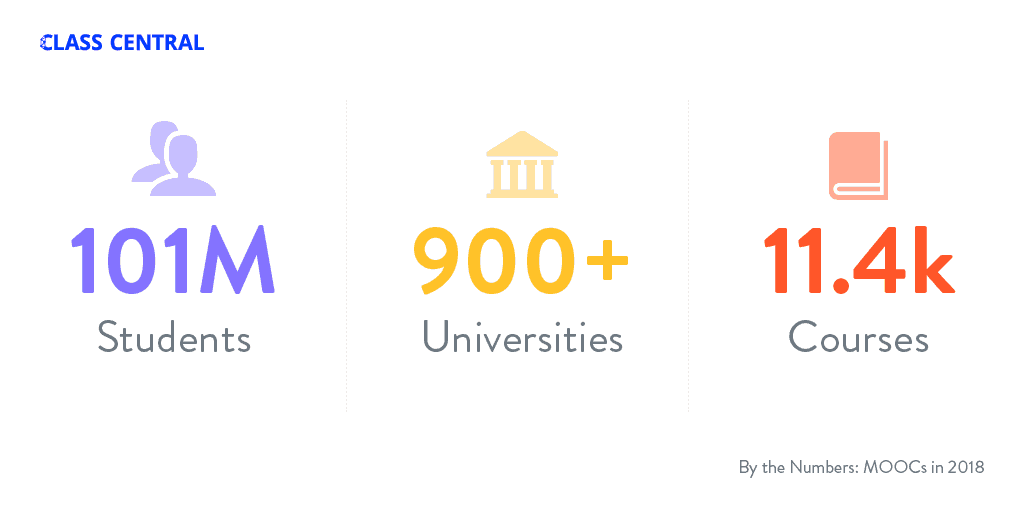
\includegraphics[scale=0.45]{stats.png}
	\caption{Overview of the online learning industry (By The Numbers: MOOCs in 2018, 2018)}	
\end{figure}
\indent
	Until this point, we discussed about online learning that is provided through the help of websites but in recent years this field has shifted to  use  mobile technology as well.  Mobile technologies are a part of our daily life and we are deeply reliant on them; Ray Kurzweil, an American inventor and futurist, even sees them as "brain extenders". There has been coined a term for learning using mobile technology, namely M-Learning, which essentially is a type of e-learning that refers to the acquisition of knowledge and skills by using mobile technologies such as smartphones, audio players or tablets. However, the most popular technology is the smartphone due to the fact that it provides other services like Internet browsing, photography, GPS, and others. Online learning through the help of online portals brings flexibility compared to traditional teaching, however, porting these online portals to mobile through native mobile applications brings even more flexibility  since the mobile device can be carried everywhere by the learner. According to Thornton and Houser (2005) a mobile learning environment increases the transfer of knowledge and feedback. Nonetheless, some suggest that mobile learning aims to improve the learning experience but should not be used as the primary method to provide a course (Wang et al. 2009). 
\newpage

\section{Mobile technologies and online learning}
   The rapid growth of mobile devices and the development of Internet mobile networks has brought online learning materials close to the learner. A lot of  people  are using their smartphones at work for private and business-related activities so it is very natural to use the phone for learning as well. 
	All the online learning platforms have developed their mobile applications in order to increase the number of learners they can reach. In order to teach a course they make use of videos with subtitles, quizzes, assignments and presentation slides. Also when using the mobile learning applications the learning content can be downloaded so offline access to it is possible. 


\subsection{Mobile Ecosystem}
%stakeholders : universities, governments, busnisess, developers, foundations, learners
	\paragraph{Digital touchpoints\\}
\indent
Users expect continuity for the online webpages (that are usually accessed in the traditional fashion by using a laptop or personal computer), namely, they want to access the webpage materials  using other devices that they possess like tablets/smartphones (through a specially tailored application). Also, very important it is to keep the webpage and mobile application synchronized regarding learning material (e.g. if a user completed an assignment on the smartphone application then it should be marked as completed on the webpage as well).\\

	\paragraph{People\\}
\indent
	The online learners represent all walks of life, from employees who have to update their skills to job seekers who are looking to sharpen their skills for the next interview. Also, students can access the online courses to get an in-depth understanding of the subjects  they are taking at university or to study courses not taught as part of their programme curriculum. Educators (e.g. teachers) can use online platforms to update their knowledge or practice flipped classroom concept (students watch the course lecture  at home and solve the assignments in the classroom where the teacher can assist them). Also, last but not least, the developers who make all this possible are part of the online learning ecosystem.\\


	\paragraph{Environments\\}
	As mentioned in the introduction, the content of the online learning platforms needs to be tailored to the learner, this can be achieved by using machine learning. Machine learning is an Artificial Intelligence technique that uses special algorithms and statistics (probabilities) to perform a specific task without being explicitly coded. Using machine learning, for instance, a questionnaire could be adapted to focus on areas where the learner might not have understood the concepts thoroughly.\\
	In order to develop mobile applications for the iOS platform a developer has to code in Objective-C or Swift. Apple provides an Integrated Development Kit (IDE) to assist the developers in the app development process, namely, Xcode. One major drawback is that if one wants to develop apps for iOS he needs a Mac laptop because iOS SDK and Xcode are available only for macOS.  Recently there were published cross-platform frameworks like Xamarin which allowed apps for iOS to be generated from a common codebase developed on Windows machine let us say. However, Apple recently changed its policy and it does not accept anymore apps that are not written using their programming languages  (Objective-C or Swift). Apart from this, once the app is developed it has to pass a tough review process in order to be published on the App Store.\\
	Android gives more flexibility to developers. In order to develop Android applications, one can use Android Studio (IDE) or Android SDK as tools for compilig the app code and as languages there can be used C++, Java or Kotlin. The Android development is not tied to any laptop or operating system, the development can be done on different operating systems (macOS, Linux or Windows). The applications can be published on the official app market of Android, namely, Google Play. Before publishing an app on the Android platform the review process is not as tough as the one that Apple performs.  However, the result of the light check before publishing an app means that the Android apps are easily hacked and injected with malware. There are other markets where one can publish Android apps but these markets do not have strong security measures in place.

\begin{figure}[H]

	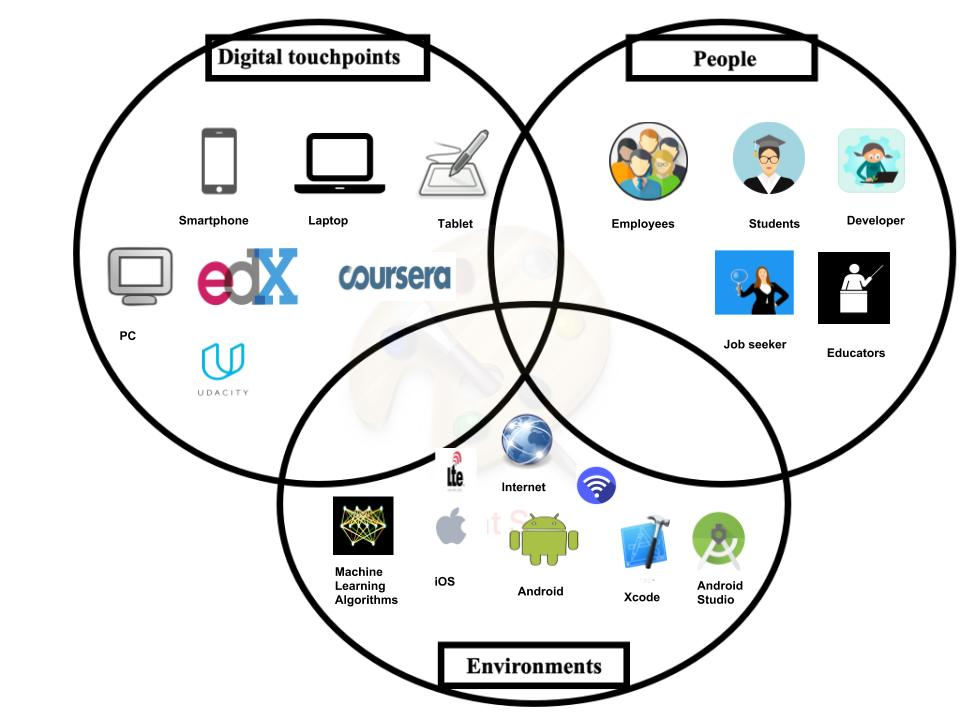
\includegraphics[scale = 0.5]{mobEco.jpg}
	\caption{The ecosystem of online learning}
	\label{onLearning}

\end{figure}

\subsection{Mobile telecommunication networks}
	Mobile telecommunication networks have been around for almost 50 years at the time of writing this work and later versions (3G, 4G) played a crucial role in the adoption of mobile computing. The first mobile telecommunication network, 1G,  started to be available to the public in 1979 (Japan) and provided basic voice service. The second communication network, 2G, was available in Europe since 1991,  represents the first digital voice service (1G was analog), improved network coverage and brought audio clarity of phone calls. Later, the development of GPRS facilitated the appearance of Internet browsers for phones. \\
	\indent
	Next, 3G, allowed broadband Internet access, mobile TV, video calls and the data speed was around 100 kb/s. However, most of the network infrastructure used by 2G  had to be replaced thus it took a long time for 3G to be globally implemented, for example, 3G was commercially launched in 2003 in the United Kingdom (UK) and only in 2007 in Kenya. In order to deploy their 3G network telecom companies had to buy licences for using a certain radio-frequency from governments. However, the market did not jump to upgrade their devices and start using the new network due to the fact that it was pretty expensive shortly after it was released. A game changer was the release of the iPhone in 2007 which was the first smartphone available to the public. The iPhone under the hood is similar to a personal computer (processing unit and memory controlled by an operating system) and at the same providing the basic the functionality of a traditional phone. The "i" in \textit{iPhone} is believed to stand for "Internet" because in their second advertisement regarding the product they referred to the iPhone as "The Internet on your phone!". To mention a few of the innovations that the iPhone brought to the world: the mass shift from keyboard input to touch input, easy software distribution and installation through a central market (App Store) and sensors embedded in the device. The market received the iPhone with a lot of enthusiasm, as can be seen in Figure~\ref{firstIphone}.\\

\begin{figure}[H]

	
\includegraphics[scale = 0.6]{iphonesMania}
	\caption{People in New York city queueing to buy the first iPhone}
	\label{firstIphone}

\end{figure} 


Nonetheless, the iPhone was pretty expensive and the people were not keen on paying extra money for mobile networks access, they were mainly using Wi-Fi to get network access. Android, launched in 2008 as a mobile operating system that powered different devices from different suppliers, made mobile computing more accessible to the large public. As a result of the development of mobile applications for the smartphone and the fact that they required higher and higher data traffic 3G started to run out of steam.\\
	\indent
	Next telecommunication network, 4G, was launched in 2009 in the Nordic countries and provides improved download/upload speed (peak download 100 Mbit/s, peak upload 50 Mbit/s), reduced latency, smooth handovers from one cell tower to another, HD video calls, HD video streaming etc. . The reduced latency from 120 ms (3G) to 75 ms (4G) makes a significant difference when playing online games or streaming live video (all social platforms provide live streaming) from a smartphone. In the past, it used to be very expensive to place a phone call from one country to another, but now, thanks to Voice over Internet Protocol (VoIP) we can make video calls for free, no wonder that WhatsApp and Skype are so popular mobile applications.\\
	\indent
	As can be observed, each new generation brings better and better services but it seems that from 4G to 5G there is the biggest leap. The data speed is expected to increase 1000 times and this will make lots of new services possible like smart cities, autonomous vehicles, 3D videos or factory automation (Osseiran et al. , 2014). The next generation, 5G, it will be launched in 2020 though  
is going to be available only in a few geographical regions initially.


\begin{figure}[H]

	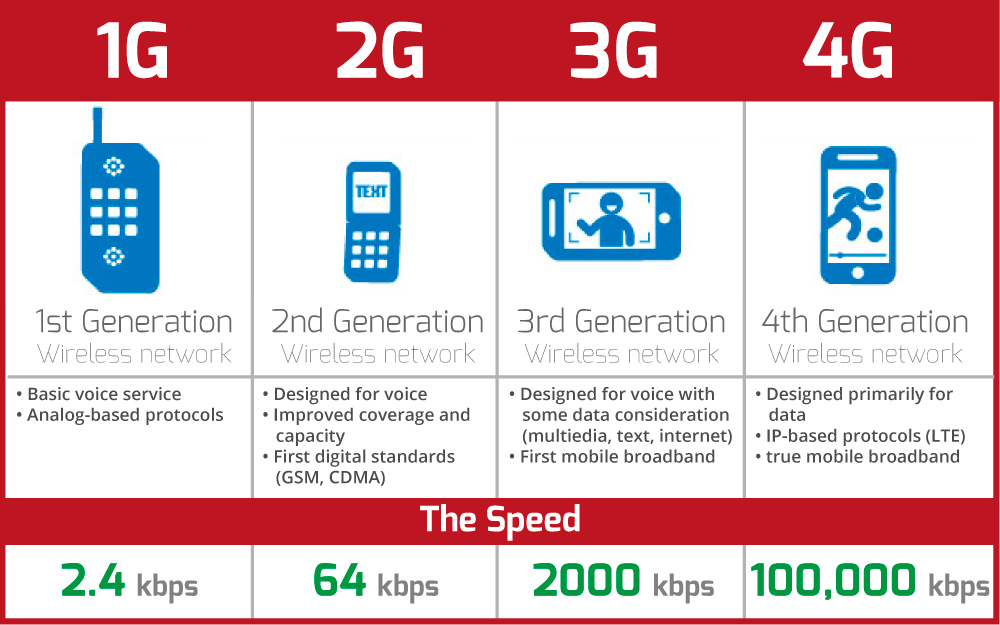
\includegraphics[scale = 0.45]{commNetworks.jpg}
	\caption{The evolution of telecommunication networks (A brief history of mobile telephony, n.d)}
	\label{commNet}

\end{figure}

\subsection{Limitations and problems}
	Simply trying to transfer classroom education to online does not seem to work, thus, new techniques have to be put in practice.
M-Learning has its own challenges which are summarized in Table~\ref{mLearChall}.


\begin{table}[H]
	\centering
	\caption{Challenges faced by M-Learning}
	\label{mLearChall}
	\begin{tabular}{|c|c|}
		\hline
		\textbf{ Challenge } & \textbf{Note}  \\
		\hline
		Lack of motivation & \makecell { Even if a company buys courses for employees they might pass\\ them by searching answers to tests on forums\\ and not by engaging with the course material}  \\	
		\hline
		Security of user & \makecell{The device needs to be carried and the individual\\ is not fully aware of what is happening around him}  \\	
		\hline
		Self-directed learning & \makecell{General concern in online learning, some of users\\ are autodidacts or advanced learners and can find\\ our own route in e-environment while others not}  \\	
		\hline
		Absence of social interaction & \makecell{Peer mentoring plays an important role in traditional education\\ and it is hard to create this in an online environment}\\
		\hline
	\end{tabular}
\end{table}

\pagebreak	
\section{Case studies: Coursera and edX}

	\subsection{Coursera}

\subsubsection{History}
	Coursera is an online for-profit learning platform that provides courses, specializations and online degrees (see Figure~\ref{courseraLogo}) for different domains like engineering, medicine or business. To create learning materials it works with an impressive number of universities (190+) and accredited individuals; the fact that it works with academia assures a high-quality of the learning materials. It was founded in 2012 by two computer scientist from Standford University, namely, Andrew Ng and Daphne Koller. The founders were inspired to create this platform because one year before founding Coursera, in 2011, they had provided online courses and managed to teach more learners than they could have had taught in an entire life in an on-campus setting. Up to this point in time the company has managed to raise \$210 million funds from different organizations. Currently, Coursera is leading the field of online learning from the perspective of registered users, having more than double compared to the next competitor (see Table~\ref{top5}). Things are good when it comes to revenue as well, Coursera's revenue for 2018 was estimated to be \$140 million and was listed in The Next-Billion Dollar Startups (2018) by Forbes. 
	\indent

\subsubsection{Mobile presence}
	In 2014, Coursera launched it's Android and iOS application in order to be able to expand their market. One of the main functionalities which the mobile application brings is the offline mode which allows one to download course content an access it while on the train or in an area without Internet connectivity. Without the mobile application, the learner is strictly dependent on Internet access and his computer.  The content of the app is well structured using tab bars with the following bar items: Explore, Recommended, Learn, Downloads and Profile. When viewing the materials for a specific course the content is organized the same using tab bars, providing the following tab items: Home, Forums, Resources, Grades and Messages. The application will be analyzed in detail in  part 2 of this report.\\

\subsubsection{Success factors}
	\indent
	Initially, courses on Coursera were session based, namely, they had a start and end date (often coinciding with fall/spring university semesters) and had deadlines for assignments. This model had several drawbacks like learners not knowing when a specific course will be offered again or the fact that different learners had different schedules. In order to address this issue in 2014 Coursera borrowed Udacity's (another online provider) idea and started to provide self-paced courses or \textit{On Demand} as they called them. The self-paced courses do not have any type of start/end date or deadlines, which allows every learner to take the course whenever they want, thus providing flexibility.  However, the problem with this approach is that there are no other learners who study the same material at the same time to have peer-discussions. Moreover, the absence of deadlines seems to discourage some learners from actively engaging with course material. Overall, the shift towards \textit{On-Demand} courses better suits Coursera because  the vast majority of its learners (users)  are professionals or "life-long learners" who look for career growth but in the same time have a busy schedule. In the past they have tried an experiment to make all the courses available for a monthly subscription but it failed so now the users pay per service.\\ 
	\indent
	In my opinion, Coursera has managed to become the leader of MOOCs industry, despite of other competitors which have been around for longer like \textit{lynda.com} founded in 1995, due to several reasons which I am going to detail. The first one  is the close tie with the academia, for example, always expanding the number of partnerships with universities (190+). The tie with academia has allowed them to tap in the know-how skills of teaching accumulated by the traditional institutions for centuries. Essentially, this helps to create a high-quality product - the online course. The second reason is the fact that it is a dynamic company, they always try to improve (as was exemplified above with the \textit{On-Demand} courses) which is absolutely necessary for the competitive online environment. Finally, their webpage is very well designed with an intuitive flow and works in good synchronization with the mobile application. In all, Coursera deserves it's leading place because it provides excellent services. 

\begin{figure}[H]

	\begin{center}
		
\includegraphics[width = 0.5\textwidth]{courseraLogo.png}
	\end{center}
	
	\caption{Coursera logo}
	\label{courseraLogo}

\end{figure}

\begin{table}[H]
	\centering
	\begin{tabular}{|c|c|c|}
		\hline
		\textbf{\#} & \textbf{Online Provider} & \textbf{\# of users} \\
		\hline
		1 & Coursera & 37 million \\
		\hline
		2 & edX      & 18 million \\
		\hline
		3 & XuetangX & 14 million \\
		\hline
		4 & Udacity & 10 million \\
		\hline
		5 & FutureLearn & 8.7 million \\
		\hline
	\end{tabular}

	\caption{Top 5 online platforms based on number of registered user (By The Numbers: MOOCs in 2018, 2018)}
	\label{top5}

\end{table}


   	\subsubsection{Monetization\\}
	The source of revenue for Coursera has mostly switched from charging per course to charge for getting certification for completion of a course, nowadays, auditing a course is (mostly) free of charge. However, there are still courses where the learner has to pay to access course materials. Other sources of revenue are specializations, online degrees and corporate training (see Table~\ref{revCoursera}). Specializations are groups of courses aimed to master a specific skill, they take between 4-6 months to complete and are priced per month (price range: \$39 USD - \$79 USD). A specialization, to give an example, like \textit{Deep Learning} is comprised of the following five courses: i) Neural Networks, ii) Improving Deep Neural Networks, iii) Structuring Machine Learning Project, iv) Convolutional Neural Networks and v) Sequence Models. Online degrees are just like traditional degrees a form of education which typically takes between 1-3 years and are taught entirely online in our case. The learner has the possibility to study for a bachelor or master degree, provided that he can afford it. These online degrees do not stick to the initial ideal of MOOCs of providing knowledge and skills at an affordable price since they are just a bit cheaper than the tuition fees that the universities charge for on-campus study; the online degrees cost between \$15 000 USD and \$25 000 USD. Like in the traditional case to enroll for an online degree the learner has to go through an admission process. To name but a few universities who provide online degrees on Coursera: University of London, Arizona State University, HEC Paris or Imperial College London. \\


	\begin{table}
		\centering
		\begin{tabular}{|c|c|c|c|}
			\hline
				\textbf{Product} & \textbf{Price Range} & \textbf{Total \# products} & \textbf{Note} \\
			\hline
				Online courses & \makecell{i) Free to audit* \\ ii) \$29 USD - \$99 USD} & 2900+ & \makecell{Two types of courses:\\
																										i) assignments not free \\
																										ii) subscription fee } \\
			\hline
				Specializations & \makecell{\$39 USD - \$79 USD \\ per month} & 250+ & \\ 
			\hline
				Online Degrees & \$15 000 USD - \$ 25 000 USD & 12 & \\
			\hline
				Corporate training & \makecell{i) \$400 USD /user/year - \\ \textbf{s}mall \textbf{o}rganization (so)\\ ii) custom pricing - \\ \textbf{l}arge \textbf{o}rganization} & \makecell{1700 \\ client employers} &  \makecell{i)so: 5 - 100 employees\\ ii)lo: over 100 employees}\\
			\hline
		\end{tabular}	
		
		\caption{Sources of revenue for Coursera (About Coursera, n.d)}
		\label{revCoursera}
	\end{table}

\pagebreak

	\subsection{edX}

\subsubsection{History}
	  The second largest online learning platform on the market is \textit{edX} (see Table~\ref{top5} ), a non-profit organization founded in 2012 with the mission to offer high-quality courses to learners around the world (see Figure~\ref{edXLogo}). It was developed by two prestigious universities from America, namely, Massachusetts Institute of Technology (MIT) and Harvard University. In contrast to Coursera's approach where a learner has to pay for coursework or quizzes, the majority of the courses on edX provide all the materials for free  and only for certification (if wanted) is perceived a fee. The organization was created with the core initiative to conduct research on learning based on how the online platform is used. The first research paper regarding learning using edX was published in 2013 once the data for their first online course, "Circuits and Electronics", was analyzed. To mention but a few of the outcomes of this research: i) it is unlikely that higher education will not be affected by MOOCs, ii) only 4\% of the enrolled learners passed the course and managed to get a certificate (high drop rate), iii) high access of the course on weekends and others (Breslow et al., 2013). There are around 130 universities that are partners with edX and a total number of 2200 online courses that edX provides.  The company has created a business plan for corporate training which in comparison with other competitors  gives analytics tools to the employers to measure employee learning engagement.
	To sum it, edX provides a more affordable approach to MOOCs than Coursera while still delivering high quality courses.\\

\subsubsection{Mobile presence}
\indent
	In 2014, edX launched it's Android and iOS application in order to be able to provide flexibility to the users since they might not have access to a personal computer all the time. The main feature of this app is the offline mode which allows the user to download the material content and use it on the go. The app provides access to all the features that the website provides (unlike Coursera's app that doesn't provide access to the forum). The content of the app is well structured using tab bars with the following bar items: i) Courses, ii) Programs and iii) Discovery. When viewing the content of a course the information is structured using the following tab items: Home, Videos, Discussion, Important Dates, Handouts and Announcements. The application will be analyzed in detail in  part 2 of this report.\\

\begin{figure}[H]

	\centering
	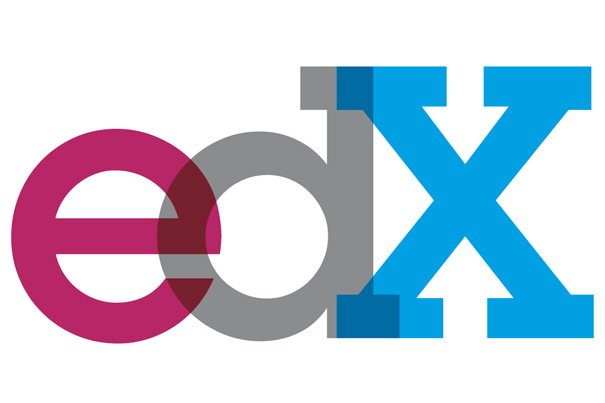
\includegraphics[width = 0.35 \textwidth]{edXLogo.jpg}
	\caption{edX company logo}
	\label{edXLogo}

\end{figure}
	\subsubsection{Monetization}
	Taking a different approach to most of the online learning platforms, namely, being a non-profit organization edX needs to find ways to sustain their organization. In 2018 they tried to enter a support fee for their services but it did not work well so starting from 2019 they require a fee tax for grading assignments. The main source of revenue for edX is the possibility to get a certification after finishing a course, the fees for a certification range between \$50 USD and \$300 USD. Apart from providing courses, just like Coursera, they provide 8 online master degrees with prices that range from \$ 10 000 USD to \$ 21 000 USD. The online master degrees are comprised on average of 10 courses and they account usually to 25\% - 50\% of credits necessary for an on-site master degree. To mention but a few universities providing online masters on edX: Georgia Tech, Univesity of Queensland or Indiana University. Another program that edX offers is \textit{MicroMaster} which provides a bundle of courses equivalent to an first term of an on-campus master programme. The good part about MicroMaster certification is that it can be used to speed up an on-campus master degree program; a MicroMaster costs between \$540 USD and \$1400 USD . Another source of revenue for edX are \textit{Professional Certificates} which are a group of courses that develop a specific skill needed in the industry. Business Writing is a  Professional Certificate comprised of the following courses: i) The Writing Process, ii) Effective Business Writing and iii) Writing for Social Media. Professional Certificates usually cost between \$120 USD and \$350 USD. Please see Table~\ref{revEdX} for an overview of some of the sources of revenue of edX.

	\begin{table}
		\begin{tabular}{|c|c|c|c|}
			\hline
			\textbf{Product} & \textbf{Price Range} & \textbf{Total  \# products} & \textbf{Note} \\
			\hline
			Online courses & \makecell{i) Free to audit \\ ii) \$50 USD - \$300 USD} & 2200 & \makecell{ i) Everything 100\% free \\ ii) certification fee} \\
			\hline 
			Online master degree & \makecell{\$ 10 000 USD - \$ 21 000 USD} & 8 & \\
			\hline 
			MicroMaster & \makecell{\$ 540 USD - \$ 1400 USD} & 52 & \\
			\hline 
			Professional Certificate & \makecell{\$ 120 USD - \$ 350 USD} & 100 & \\
			\hline 
		\end{tabular}
		\caption{Sources of revenue for edX}
		\label{revEdX}
	\end{table}

%FIXME maybe do a comparison of the two learning platforms using Alexa.com info - to add some words
\newpage
\section{References}
A brief history of mobile telephony. (n.d.) Available: http://smartipx.com/brief-history-mobile-telephony/ [Accessed: 7 March 2019].\\

About Coursera. (n.d.) Available: https://about.coursera.org/ [Accessed: 1 March 2019].\\

Bloom, B.S., 1984. The 2 sigma problem: The search for methods of group instruction as effective as one-to-one tutoring. Educational researcher, 13(6), pp.4-16. \\

Breslow, L., Pritchard, D.E., DeBoer, J., Stump, G.S., Ho, A.D. and Seaton, D.T., 2013. Studying learning in the worldwide classroom research into edX's first MOOC. Research \& Practice in Assessment, 8, pp.13-25.\\

By The Numbers: MOOCs In 2018. (2018) Available: https://www.class-central.com/report/mooc-stats-2018/ [Accessed: 27 February 2019]\\


Wang, Y.S., Wu, M.C. and Wang, H.Y., 2009. Investigating the determinants and age and gender differences in the acceptance of mobile learning. British journal of educational technology, 40(1), pp.92-118.\\

Hamidi, H. and Chavoshi, A., 2018. Analysis of the essential factors for the adoption of mobile learning in higher education: A case study of students of the University of Technology. Telematics and Informatics, 35(4), pp.1053-1070.\\

Mazoué, J.G., 2012. The deconstructed campus. Journal of Computing in Higher Education, 24(2), pp.74-95.\\

Osseiran, A., Boccardi, F., Braun, V., Kusume, K., Marsch, P., Maternia, M., Queseth, O., Schellmann, M., Schotten, H.D., Hidekazu, T. and Tullberg, H.M., 2014. Scenarios for 5G mobile and wireless communications: The vision of the METIS project. IEEE Communications Magazine, 52(5), pp.26-35.\\

The Next Billion-Dollar Startups (2018)\\
 Available: https://www.forbes.com/next-billion-dollar-startups/\#246a9dbe4441 [Accessed: 28 February 2019].\\

Thornton, P. and Houser, C., 2005. Using mobile phones in English education in Japan. Journal of computer assisted learning, 21(3), pp.217-228.\\

Wang, Y.S., Wu, M.C. and Wang, H.Y., 2009. Investigating the determinants and age and gender differences in the acceptance of mobile learning. British journal of educational technology, 40(1), pp.92-118.\\

Wessel, M. and Christensen, C.M., 2012. Surviving disruption. Harvard Business Review, 90(12), pp.56-64.\\

\end{document}

